\chapter{Microtubule Structure \& Function}
\label{ch:microtubule-structure-function}

\textbf{Microtubules are the ``scaffolding'' of your cells}---tiny hollow tubes made of proteins that give cells their shape and move things around. They're incredibly small: 25 nanometers wide (1/4000th the width of a human hair).

\textbf{What they definitely do:}
\begin{itemize}
\item \textbf{Structural support:} Like steel beams, they keep cells rigid
\item \textbf{Transportation highways:} Roads for ``molecular trucks'' (motor proteins)
\item \textbf{Cell division:} Pull chromosomes apart during cell division
\item \textbf{Movement:} Form the core of sperm tails and lung cilia
\end{itemize}

\textbf{The quantum controversy:} Some scientists propose that microtubules in brain cells might use quantum mechanics to process information or even generate consciousness. This is \emph{highly speculative}---most neuroscientists are skeptical because brains are too warm and wet for quantum effects (which usually need extreme cold and isolation).

\textbf{Current status:} Microtubules are essential for cell function (proven). Whether they do anything quantum-related in the brain remains an open question requiring better experiments.
\section{Overview}

\textbf{Microtubules} are cylindrical protein polymers (25~nm diameter, 15~nm lumen) that form part of the cytoskeleton in eukaryotic cells. They consist of $\alpha$-$\beta$ tubulin heterodimers polymerized into 13 protofilaments arranged in a hollow tube.

\begin{keyconcept}
Microtubules perform \textbf{established biological functions} (structural support, intracellular transport, cell division) with well-understood classical mechanics. The hypothesis that they enable \textbf{quantum information processing in neurons} remains highly speculative and controversial.
\end{keyconcept}

\textbf{Established roles:}
\begin{itemize}
\item Structural support (Young's modulus $\sim$1--2~GPa)
\item Intracellular transport (kinesin and dynein motor tracks)
\item Cell division (mitotic spindle formation)
\item Cilia and flagella (9+2 axoneme motility)
\end{itemize}

\textbf{Speculative quantum roles:}
\begin{itemize}
\item Quantum computation substrates (unproven)
\item Consciousness generation via Orch-OR theory (controversial)
\item Information integration beyond classical neural networks (no experimental evidence)
\end{itemize}

\section{Molecular Structure and Assembly}

\subsection{Tubulin Dimers}

The fundamental building block of microtubules is the $\alpha$-$\beta$ tubulin heterodimer:

\textbf{Composition:}
\begin{itemize}
\item \textbf{$\alpha$-tubulin}: 451 amino acids, $\sim$50~kDa, globular protein
\item \textbf{$\beta$-tubulin}: 445 amino acids, $\sim$50~kDa, globular protein
\item \textbf{Dimer dimensions}: 8~nm long, 4~nm diameter
\item \textbf{GTP binding}: Both subunits have nucleotide-binding sites; $\beta$-tubulin is hydrolysis-active
\end{itemize}

\textbf{Key structural features:}
\begin{itemize}
\item \textbf{Aromatic residues}: 16 Trp, 25 Tyr, 39 Phe per dimer (potential quantum chromophores in speculative theories)
\item \textbf{Hydrophobic core}: Stabilizes folded structure
\item \textbf{C-terminal tail}: Acidic, flexible, extends from surface ($\sim$15 amino acids)
\end{itemize}

The tubulin dimer structure was resolved to 3.5~Å resolution by Nogales et al.~(1998), providing the molecular basis for understanding microtubule assembly.

\subsection{Protofilaments and Lattice Architecture}

\textbf{Assembly hierarchy:}
\begin{enumerate}
\item Tubulin dimers polymerize head-to-tail $\rightarrow$ \textbf{protofilament}
\item 13 protofilaments associate laterally $\rightarrow$ cylindrical microtubule
\end{enumerate}

\textbf{Geometric parameters:}
\begin{equation}
D_{\mathrm{outer}} = 25\ \mathrm{nm}, \quad D_{\mathrm{inner}} = 15\ \mathrm{nm}, \quad t_{\mathrm{wall}} = 5\ \mathrm{nm}
\end{equation}
where:
\begin{itemize}
\item $D_{\mathrm{outer}}$ = outer diameter
\item $D_{\mathrm{inner}}$ = inner (lumen) diameter
\item $t_{\mathrm{wall}}$ = wall thickness
\end{itemize}

\begin{center}
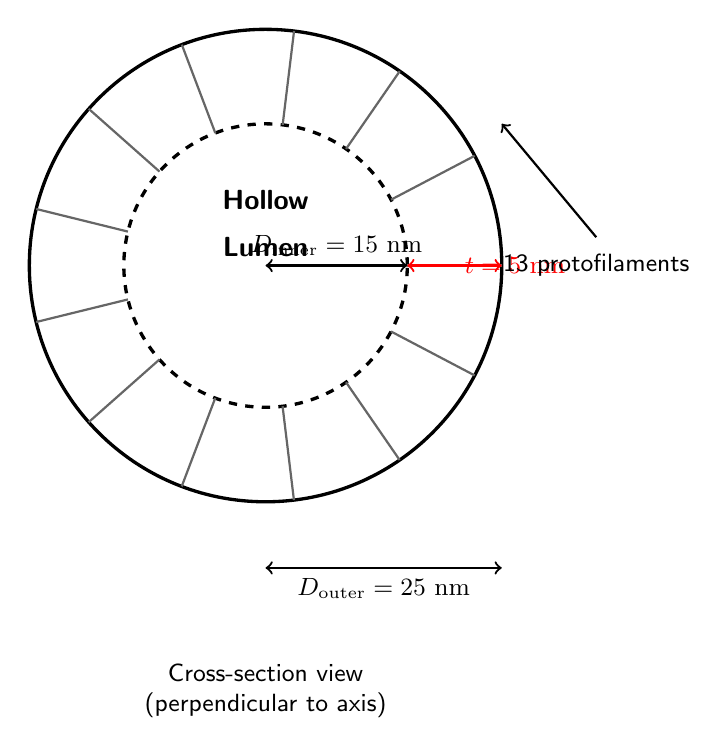
\begin{tikzpicture}[scale=1.2]
% Cross-section view of microtubule
\draw[very thick] (0,0) circle (2.5cm);
\draw[very thick,dashed] (0,0) circle (1.5cm);

% 13 protofilaments (represented as radial segments)
\foreach \angle in {0,27.69,...,360} {
    \draw[thick,black!60] (\angle:1.5cm) -- (\angle:2.5cm);
}

% Dimensions
\draw[<->,thick] (0,0) -- node[above,font=\small] {$D_{\mathrm{inner}}=15$~nm} (1.5,0);
\draw[<->,thick] (0,-3.2) -- node[below,font=\small] {$D_{\mathrm{outer}}=25$~nm} (2.5,-3.2);
\draw[<->,thick,red] (0:1.5) -- node[right,font=\small,red] {$t=5$~nm} (0:2.5);

% Labels
\node[font=\sffamily\bfseries] at (0,0.7) {Hollow};
\node[font=\sffamily\bfseries] at (0,0.2) {Lumen};
\node[font=\sffamily\small] at (3.5,0) {13 protofilaments};
\draw[->,thick] (3.5,0.3) -- (2.5,1.5);

% Tubulin dimers indicator
\node[font=\sffamily\small,align=center] at (0,-4.5) {Cross-section view\\(perpendicular to axis)};
\end{tikzpicture}
\end{center}

\textbf{Helical geometry:}
\begin{itemize}
\item \textbf{Helical pitch}: $h = 12.5$~nm (3-start helix for 13-protofilament structure)
\item \textbf{Lattice seam}: Lateral contacts slightly different at one position (breaks rotational symmetry)
\item \textbf{Polarity}: Plus end ($\beta$-tubulin exposed) vs.~minus end ($\alpha$-tubulin exposed)
\end{itemize}

\textbf{Lattice types:}
\begin{itemize}
\item \textbf{A-lattice}: Straight protofilaments, perfect alignment (most common in vivo)
\item \textbf{B-lattice}: Helical protofilaments, staggered alignment (some in vitro conditions)
\end{itemize}

\subsection{Dynamic Instability}

\textbf{Phenomenon:} Microtubules stochastically switch between growth and rapid shrinkage---a behavior discovered by Mitchison \& Kirschner (1984) that is fundamental to cytoskeletal reorganization.

\textbf{Mechanism:}
\begin{enumerate}
\item \textbf{GTP cap}: Newly added tubulin dimers have GTP bound to $\beta$-tubulin
\item \textbf{Hydrolysis}: GTP $\rightarrow$ GDP after incorporation (delayed by $\tau_{\mathrm{hyd}} \sim 1$~s)
\item \textbf{Catastrophe}: If GTP cap is lost, GDP-tubulin (unstable) is exposed $\rightarrow$ rapid depolymerization
\item \textbf{Rescue}: Occasional stabilization events re-establish growth
\end{enumerate}

\begin{center}
\begin{tikzpicture}[scale=1.0,
  state/.style={rectangle,draw,thick,minimum width=2.5cm,minimum height=1cm,font=\sffamily\small},
  node distance=3.5cm]
  
\node[state] (growth) {GROWTH\\$v_+ \sim 2$ $\mu$m/min};
\node[state,right of=growth] (shrink) {SHRINKAGE\\$v_- \sim 15$ $\mu$m/min};

\draw[->,thick,bend left=30] (growth) to node[above,font=\scriptsize] {Catastrophe ($f_{\mathrm{cat}} \sim 0.01$ s$^{-1}$)} (shrink);
\draw[->,thick,bend left=30] (shrink) to node[below,font=\scriptsize] {Rescue ($f_{\mathrm{res}} \sim 0.001$ s$^{-1}$)} (growth);

% Annotations
\node[below=0.2cm of growth,font=\small,align=center] {GTP cap\\stable};
\node[below=0.2cm of shrink,font=\small,align=center] {GDP exposed\\unstable};

\node[above=1.5cm of growth,xshift=1.5cm,font=\sffamily\small,align=left] {Parameters (in vitro, 37$^\circ$C):};
\end{tikzpicture}
\end{center}

\textbf{Quantitative parameters} (in vitro, 37$^\circ$C):

\begin{equation}
v_+ = 2\ \mu\mathrm{m/min}, \quad v_- = 10\text{--}20\ \mu\mathrm{m/min}
\end{equation}
\begin{equation}
f_{\mathrm{cat}} = 0.01\ \mathrm{s}^{-1}, \quad f_{\mathrm{res}} = 0.001\ \mathrm{s}^{-1}
\end{equation}
where:
\begin{itemize}
\item $v_+$ = growth velocity (plus-end)
\item $v_-$ = shrinkage velocity
\item $f_{\mathrm{cat}}$ = catastrophe frequency
\item $f_{\mathrm{res}}$ = rescue frequency
\end{itemize}

\textbf{Biological function:} Dynamic instability enables rapid cytoskeletal reorganization during mitosis, cell migration, and axon guidance.

\subsection{2. Cellular Functions (Established
)}\label{cellular-functions-established}

\subsubsection{2.1 Structural Support}\label{structural-support}

Microtubules provide mechanical rigidity to cells through their exceptional stiffness:

\textbf{Young's modulus:}
\begin{equation}
E = 1\text{--}2\ \mathrm{GPa}
\end{equation}
where $E$ is Young's modulus (stiffer than actin filaments at $\sim$2~MPa).

\textbf{Persistence length:}
\begin{equation}
L_p = \frac{EI}{k_B T} \approx 5\ \mathrm{mm}
\end{equation}
where:
\begin{itemize}
\item $L_p$ = persistence length (measure of bending stiffness)
\item $I$ = second moment of area (hollow cylinder geometry)
\item $k_B$ = Boltzmann constant ($1.38 \times 10^{-23}$~J/K)
\item $T$ = absolute temperature (K)
\end{itemize}

\textbf{Buckling force:}
\begin{equation}
F_{\mathrm{buckle}} = \frac{\pi^2 EI}{L^2} \approx 5\ \mathrm{pN}
\end{equation}
where $L$ is the length of the microtubule segment.

\begin{calloutbox}{Physical Interpretation}
A persistence length of $L_p \sim 5$~mm is enormous compared to typical cell dimensions (10--100~$\mu$m), meaning microtubules are essentially rigid rods on cellular scales. This rigidity enables them to maintain cell shape and resist compressive loads.
\end{calloutbox}

\subsection{Intracellular Transport}

Microtubules serve as tracks for molecular motor proteins that transport cargo throughout the cell.

\textbf{Motor proteins:}
\begin{itemize}
\item \textbf{Kinesin}: Moves toward plus end (anterograde transport in axons)
\item \textbf{Dynein}: Moves toward minus end (retrograde transport)
\end{itemize}

\textbf{Motor performance:}
\begin{equation}
v_{\mathrm{motor}} \approx 1\ \mu\mathrm{m/s}, \quad F_{\mathrm{motor}} \approx 5\text{--}7\ \mathrm{pN}
\end{equation}
where:
\begin{itemize}
\item $v_{\mathrm{motor}}$ = motor velocity
\item $F_{\mathrm{motor}}$ = stall force (maximum pulling force)
\end{itemize}

\textbf{Cargo:} Vesicles, mitochondria, mRNA granules, protein complexes

\begin{importantbox}
\textbf{Medical relevance:} Defects in axonal transport are linked to neurodegenerative diseases including Alzheimer's disease and amyotrophic lateral sclerosis (ALS). Disrupted cargo transport leads to accumulation of toxic proteins and organelle dysfunction.
\end{importantbox}

\subsection{Mitotic Spindle}

\textbf{Function:} Segregate chromosomes during cell division with high fidelity.

\textbf{Structure:}
\begin{itemize}
\item \textbf{Astral microtubules}: Extend from centrosomes to cell cortex
\item \textbf{Kinetochore microtubules}: Attach to chromosomes
\item \textbf{Interpolar microtubules}: Overlap at spindle midzone
\end{itemize}

\textbf{Force generation:}
\begin{equation}
F_{\mathrm{chrom}} \approx 10\ \mathrm{pN}
\end{equation}
where $F_{\mathrm{chrom}}$ is the force exerted on each chromosome by depolymerizing kinetochore microtubules.

\subsection{Cilia and Flagella}

\textbf{Structure:} \textbf{9+2 axoneme} (9 doublet microtubules + 2 central singlets)

\textbf{Mechanism:} Dynein arms on doublets cause sliding $\rightarrow$ bending motion

\textbf{Beat frequency:}
\begin{equation}
f_{\mathrm{beat}} = 10\text{--}60\ \mathrm{Hz}
\end{equation}
where $f_{\mathrm{beat}}$ depends on cilium/flagellum type and physiological conditions.

\textbf{Examples:}
\begin{itemize}
\item \textbf{Respiratory cilia}: Clear mucus from airways (10--20~Hz)
\item \textbf{Sperm flagella}: Propulsion ($\sim$60~Hz beat frequency)
\item \textbf{Nodal cilia}: Establish left-right asymmetry in embryos
\end{itemize}

\section{Neural Microtubules: Unique Features}

\subsection{Neuronal Cytoskeleton Organization}

\textbf{Axons:}
\begin{itemize}
\item Microtubules uniformly oriented (plus-ends distal)
\item Continuous tracks for kinesin transport
\item Stabilized by tau protein (hyperphosphorylation in Alzheimer's disease)
\end{itemize}

\textbf{Dendrites:}
\begin{itemize}
\item Mixed polarity microtubules
\item Both kinesin and dynein active
\item Dynamic remodeling during synaptic plasticity
\end{itemize}

\textbf{Microtubule density:}
\begin{equation}
N_{\mathrm{MT}} \sim 10^6\ \text{microtubules per neuron}
\end{equation}
where $N_{\mathrm{MT}}$ varies with neuron type and maturation state.

\subsection{Post-Translational Modifications (PTMs)}

\textbf{Tubulin code:} $\sim$20 different PTMs create functional diversity, analogous to the histone code in chromatin.

\textbf{Key modifications:}
\begin{itemize}
\item \textbf{Acetylation} (Lys-40 on $\alpha$-tubulin): Marks stable, long-lived microtubules
\item \textbf{Tyrosination/detyrosination}: Regulates motor protein binding
\item \textbf{Polyglutamylation}: C-terminal tail modification (affects MAP binding)
\item \textbf{Phosphorylation}: Tau phosphorylation regulates microtubule stability
\end{itemize}

\textbf{Function:} PTMs create binding codes for MAPs (microtubule-associated proteins), motors, and signaling proteins, enabling context-dependent regulation of cytoskeletal function.

\subsection{Microtubule-Associated Proteins (MAPs)}

\textbf{Major MAP families:}
\begin{itemize}
\item \textbf{Tau}: Stabilizes microtubules (predominantly in axons)
\item \textbf{MAP2}: Stabilizes microtubules (predominantly in dendrites)
\item \textbf{MAP4}: Ubiquitous stabilizer
\item \textbf{EB proteins}: Track plus-ends (regulate dynamics)
\end{itemize}

\begin{importantbox}
\textbf{Anesthetic sensitivity:} General anesthetics (isoflurane, propofol) bind to tubulin and disrupt MAP interactions $\rightarrow$ altered microtubule dynamics. This correlation with loss of consciousness is cited in support of microtubule-based consciousness theories, though classical explanations (disrupted synaptic function) remain more parsimonious.
\end{importantbox}

\subsection{4. Quantum Biology Hypotheses (Speculative
)}\label{quantum-biology-hypotheses-speculative}

\subsubsection{4.1 Orch-OR Theory
(Penrose-Hameroff)}\label{orch-or-theory-penrose-hameroff}

\textbf{Core claim}: Consciousness arises from quantum computations in
microtubules, terminated by objective reduction (OR).

\textbf{Mechanism} (proposed): 1. Tubulin dimers exist in superposed
states (conformational states or electronic states) 2. Quantum coherence
spreads across
\textasciitilde10\textbackslash textsuperscript\{5\}-10\textbackslash textsuperscript\{7\}
tubulins via dipole-dipole interactions 3. Superposition reaches OR
threshold: \(E \cdot \tau \sim \hbar\) (energy \$\textbackslash times\$
time \textasciitilde{} Planck constant) 4. Wavefunction collapses
\$\textbackslash rightarrow\$ conscious moment (\textasciitilde25 ms,
gamma oscillation period)

\textbf{Requirements}: - Coherence time \(\tau_c > 1\) ms at 310 K -
Isolation from environment (ordered water shell?) - Quantum-to-classical
interface (how does OR generate neural firing?)

\textbf{Status}: No experimental confirmation; decoherence estimates
vary wildly (femtoseconds to milliseconds)

\subsubsection{4.2 Quantum Information
Processing}\label{quantum-information-processing}

\textbf{Hypothesis}: Microtubules perform quantum computations beyond
classical neuron networks.

\textbf{Encoding schemes} (speculative): - \textbf{Conformational
qubits}: Tubulin dimer in superposition of two conformations -
\textbf{Electronic qubits}: Aromatic amino acids in superposed
\(\pi\)-electron states - \textbf{Phononic qubits}: THz vibrational
modes (see {[}{[}THz-Resonances-in-Microtubules{]}{]})

\textbf{Entanglement propagation}: - Nearest-neighbor dipole coupling:
\(V_{ij} \sim 10^{-3}\) eV (weak but non-zero) - Coherent
phonon-mediated coupling: Possible if Fröhlich condensate exists

\textbf{Computational advantage}: Quantum parallelism
\$\textbackslash rightarrow\$ exponential speed-up for certain tasks
(e.g., pattern recognition?)

\textbf{Problem}: No known biological algorithm requires quantum
computation; classical neural networks already very powerful

\subsubsection{4.3 Vibronic Coherence at Room
Temperature}\label{vibronic-coherence-at-room-temperature}

\textbf{Insight from VE-TFCC theory}: - Strong vibronic coupling
(electron-phonon interaction) can sustain thermal quantum coherence -
Bogoliubov quasiparticles diagonalize thermal Hamiltonian
\$\textbackslash rightarrow\$ stable coherent states at 310 K

\textbf{Application to microtubules}: - Aromatic residues (Trp, Tyr,
Phe) have \(\pi\)-electron systems - Couple to THz lattice vibrations
\$\textbackslash rightarrow\$ vibronic excitations - If coupling
strength \(g \omega \gtrsim k_B T\), coherence survives

\textbf{Testable prediction}: Measure quantum variance
\(\langle q^2 \rangle - \langle q \rangle^2\) in microtubules; excess
variance (beyond classical thermal) indicates quantum coherence

\textbf{Status}: Not yet measured experimentally

\begin{center}\rule{0.5\linewidth}{0.5pt}\end{center}

\subsection{5. Critical Challenges to Quantum
Hypotheses}\label{critical-challenges-to-quantum-hypotheses}

\subsubsection{5.1 Decoherence Problem}\label{decoherence-problem}

\textbf{Tegmark\textquotesingle s calculation} (2000): Decoherence time
\(\tau_d \sim 10^{-13}\) s (100 femtoseconds) due to: - Water dielectric
fluctuations - Ion motion (Na\textbackslash textsuperscript\{+\},
K\textbackslash textsuperscript\{+\},
Ca\textbackslash textsuperscript\{2\}\textbackslash textsuperscript\{+\})
- Thermal phonons

\textbf{Counter-arguments}: - Tegmark assumed point dipoles; extended
wavefunction may decohere slower - Ordered water near microtubule
surface reduces fluctuations - Vibronic coupling creates
decoherence-free subspaces (VE-TFCC insight)

\textbf{Current status}: No consensus; experimental measurement needed

\subsubsection{5.2 Lack of Biological
Function}\label{lack-of-biological-function}

\textbf{Evolutionary argument}: If quantum effects were functionally
important, we\textquotesingle d expect: - Selection pressure to maintain
coherence (e.g., specialized shielding proteins) - Deficits in organisms
lacking microtubules (but prokaryotes have cognition without
microtubules)

\textbf{Alternative explanation}: All known neural functions explainable
by classical electrophysiology

\subsubsection{5.3 Anesthetic Paradox}\label{anesthetic-paradox}

\textbf{Observation}: General anesthetics disrupt consciousness and bind
to microtubules.

\textbf{Quantum interpretation}: Anesthetics disrupt THz coherence
\$\textbackslash rightarrow\$ loss of quantum computation
\$\textbackslash rightarrow\$ unconsciousness

\textbf{Classical interpretation}: Anesthetics alter microtubule-MAP
interactions \$\textbackslash rightarrow\$ disrupt synaptic vesicle
transport \$\textbackslash rightarrow\$ loss of neurotransmission

\textbf{Test}: Does anesthetic binding shift THz resonances or reduce
coherence times? - \textbf{Preliminary data} (in vitro): Yes, small
shifts (\textasciitilde0.1 THz) - \textbf{In vivo test}: Not yet done

\begin{center}\rule{0.5\linewidth}{0.5pt}\end{center}

\subsection{6. Experimental Frontiers}\label{experimental-frontiers}

\subsubsection{6.1 What Would Prove Quantum
Function?}\label{what-would-prove-quantum-function}

Requires demonstrating: 1. \textbf{Long-lived coherence}: \(\tau_c > 1\)
ms at 310 K in functioning neurons 2. \textbf{Functional relevance}:
Disrupting coherence impairs cognition in specific, predictable ways 3.
\textbf{Quantum advantage}: A task neurons perform that classical
systems provably cannot

\subsubsection{6.2 Proposed Experiments}\label{proposed-experiments}

\textbf{THz spectroscopy}: - Two-dimensional THz on microtubules (detect
off-diagonal coherences) - Temperature dependence (does coherence vanish
classically at high \(T\)?)

\textbf{Isotope effects}: - Deuterate tubulin (H
\$\textbackslash rightarrow\$ D changes vibrational frequencies) -
Predict altered coherence times \$\textbackslash rightarrow\$ test with
cognitive assays

\textbf{Quantum sensors}: - NV-diamond magnetometry: Detect weak
magnetic fields from radical pairs in tubulin - SQUID arrays: Map
magnetic coherence in brain slices

\begin{center}\rule{0.5\linewidth}{0.5pt}\end{center}

\subsection{7. Connections to Other Wiki
Pages}\label{connections-to-other-wiki-pages}

\begin{itemize}
\tightlist
\item
  {[}{[}Orchestrated-Objective-Reduction-(Orch-OR){]}{]} -\/-\/-
  Consciousness theory requiring microtubule quantum effects
\item
  {[}{[}Quantum-Coherence-in-Biological-Systems{]}{]} -\/-\/- General
  framework
\item
  {[}{[}THz-Resonances-in-Microtubules{]}{]} -\/-\/- Vibrational modes
  that could sustain coherence
\item
  {[}{[}Terahertz-(THz)-Technology{]}{]} -\/-\/- Experimental probes
\item
  {[}{[}Hyper-Rotational-Physics-(HRP)-Framework{]}{]} -\/-\/-
  Theoretical extension to consciousness
\end{itemize}

\begin{center}\rule{0.5\linewidth}{0.5pt}\end{center}

\subsection{8. References}\label{references}

\subsubsection{Structure and Function
(Established)}\label{structure-and-function-established}

\begin{enumerate}
\def\labelenumi{\arabic{enumi}.}
\tightlist
\item
  \textbf{Nogales et al., \emph{Nature} 391, 199 (1998)} -\/-\/- Tubulin
  crystal structure
\item
  \textbf{Mitchison \& Kirschner, \emph{Nature} 312, 237 (1984)} -\/-\/-
  Dynamic instability discovery
\item
  \textbf{Desai \& Mitchison, \emph{Annu. Rev.~Cell Dev. Biol.} 13, 83
  (1997)} -\/-\/- Microtubule dynamics review
\end{enumerate}

\subsubsection{Quantum Hypotheses
(Speculative)}\label{quantum-hypotheses-speculative}

\begin{enumerate}
\def\labelenumi{\arabic{enumi}.}
\setcounter{enumi}{3}
\tightlist
\item
  \textbf{Penrose \& Hameroff, \emph{Phys. Life Rev.} 11, 39 (2014)}
  -\/-\/- Orch-OR consciousness theory
\item
  \textbf{Hameroff \& Penrose, \emph{J. Conscious. Stud.} 21, 126
  (2014)} -\/-\/- Orch-OR update
\end{enumerate}

\subsubsection{Critical Perspectives}\label{critical-perspectives}

\begin{enumerate}
\def\labelenumi{\arabic{enumi}.}
\setcounter{enumi}{5}
\tightlist
\item
  \textbf{Tegmark, \emph{Phys. Rev.~E} 61, 4194 (2000)} -\/-\/-
  Decoherence calculation (skeptical)
\item
  \textbf{Koch \& Hepp, \emph{Nature} 440, 611 (2006)} -\/-\/- Critique
  of quantum consciousness
\end{enumerate}

\subsubsection{Vibronic Coupling}\label{vibronic-coupling}

\begin{enumerate}
\def\labelenumi{\arabic{enumi}.}
\setcounter{enumi}{7}
\tightlist
\item
  \textbf{Bao et al., \emph{J. Chem. Theory Comput.} 20, 4377 (2024)}
  -\/-\/- VE-TFCC theory (thermal coherence)
\end{enumerate}

\begin{center}\rule{0.5\linewidth}{0.5pt}\end{center}

\textbf{Last updated}: October 2025
